\documentclass{article}
\title{Logical and Physical Database Design}
\author{Claire Trebing, Jason Young, Illya Starikov}
\date{Due Date: March 18, 2016}

\usepackage{pdfpages}
\usepackage{graphicx}
\usepackage{multicol}
\usepackage{amsmath}
\usepackage{changepage}
\usepackage{booktabs}
\usepackage[shortlabels]{enumitem}
% \usepackage[showframe=true]{geometry}

\newcommand{\pk}{$^{\text{\textbf{PK}}}$}
\newcommand{\fk}{$^{\text{\textit{FK}}}$}
\newcommand{\pfk}{$^{\text{\textit{\textbf{PK, FK}}}}$}

\newcommand{\br}{\multicolumn{2}{c}{} \\}

\begin{document}
\maketitle

\section{Revised Problem Statement}
2015 marked a record year for Americans regularly exercising, hitting just over 55\%. Keeping that momentum is difficult. As blue-collar jobs continue to decline, it has been more important than ever to keep a weekly regimen of healthy eating and exercising.

Living in the most interconnected generation poses quite a viable idea for social networking: healthy living. We can build a social network that connects users to friends, peers and family to make an online community of healthy living.

Our database will be essential because it will unite something so mundane and uninteresting with familiar faces. This will make exercise more enjoyable and offer a group to hold you accountable. We can shape an entire generation by having motivation a click away.

This database will consist of premade workouts, groups, and reminder emails to help you stay on top of your fitness plan.

\section{Revised Conceptual Database Design}
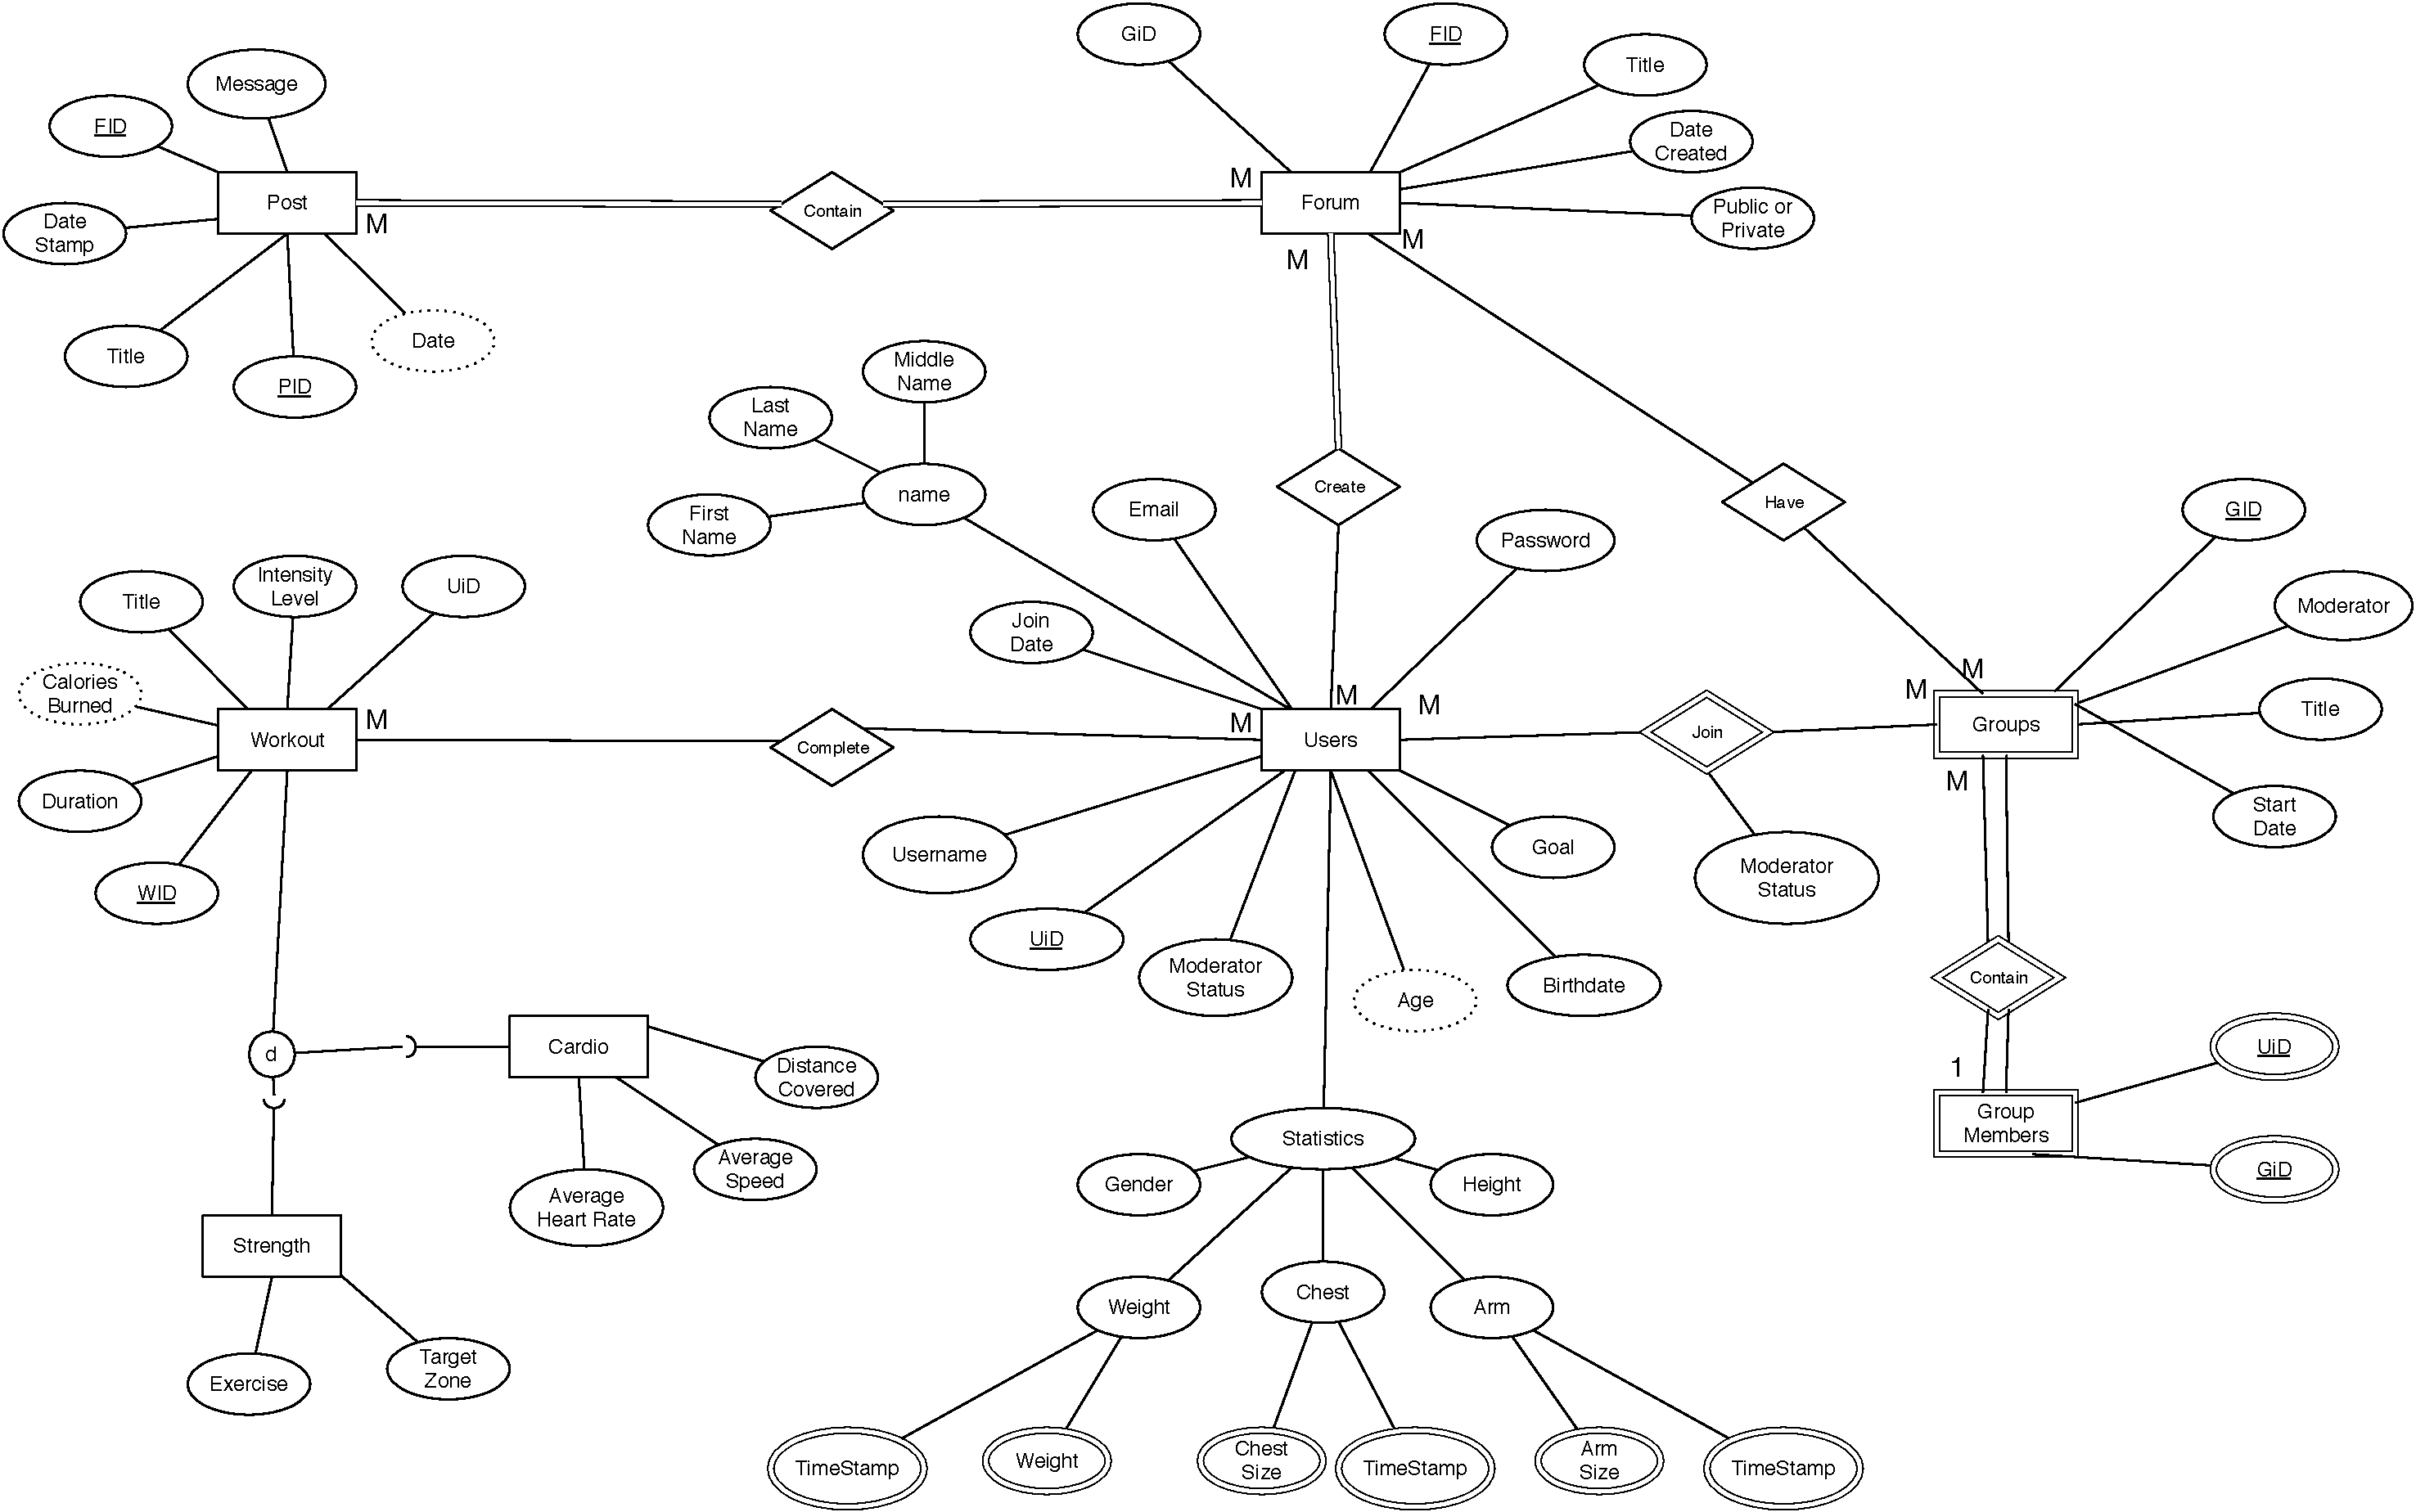
\includepdf[pages=-,width=1.75\textwidth]{EER_Diagram_(Phase_II).pdf}

\section{Logical Database Design}
\subsection{Relational Set}
Please note primary keys are signified by \pk \ and foreign keys are signified by \fk.

%-------------------- Post --------------------%
\subsection*{Post}
\begin{tabular}{|l|l|l|l|l|l|}
\hline
\underline{PiD} \pk & \underline{FiD} \fk & Message & DateStamp & Title & Date \\
\hline
\end{tabular}

%-------------------- Forum --------------------%
\subsection*{Forum}
\begin{tabular}{|l|l|l|l|l|l|}
\hline
\underline{FiD} \pk & Title & DateCreated & PublicOrPrivate & GiD \fk \\
\hline
\end{tabular}

%-------------------- Groups --------------------%
\subsection*{Groups}
\begin{tabular}{|l|l|l|l|l|}
\hline
\underline{GiD} \pk & Moderator \fk & Title & StartDate  \\
\hline
\end{tabular}

%-------------------- Workout --------------------%
\subsection*{Workouts}
\begin{tabular}{|l|l|l|l|l|l|}
\hline
\underline{WiD} \pk & Duration & Title & IntensityLevel & CaloriesBurned & UiD \fk \\
\hline
\end{tabular}

%-------------------- Strength --------------------%
\subsection*{Strength}
\begin{tabular}{|l|l|l|l|l|l|l|l|}
\hline
\underline{WiD} \pk & Duration & Title & IntensityLevel & CaloriesBurned & UiD \fk & Exercise & Target Zone \\
\hline
\end{tabular}

%-------------------- Cardio --------------------%
\subsection*{Cardio}
\begin{tabular}{|l|l|l|l|l|l|l|}
\hline
\underline{WiD} \pk & Duration & Title & IntensityLevel & CaloriesBurned & UiD \fk & AverageHeartRate \\
\hline
\end{tabular}
\begin{tabular}{|l|l|}
\hline
AverageSpeed & DistanceCovered \\
\hline
\end{tabular}

%-------------------- Cardio --------------------%
\subsection*{Users}
\begin{tabular}{|l|l|l|l|l|l|l|l|l|}
\hline
\underline{UiD} \pk & Username & Height & Birthdate & Goal & Password & JoinDate & Gender\\
\hline
\end{tabular}
\begin{tabular}{|l|l|l|}
\hline
FirstName & MiddleName & LastName \\
\hline
\end{tabular}

\begin{multicols}{2}
%-------------------- Weight --------------------%
\subsection*{Weight}
\begin{tabular}{|l|l|l|}
\hline
\underline{UiD} \pfk & \underline{TimeStamp} \pk & Weight \\
\hline
\end{tabular}

%-------------------- Chest Size --------------------%
\subsection*{Chest Size}
\begin{tabular}{|l|l|l|}
\hline
\underline{UiD} \pfk & \underline{TimeStamp} \pk & ChestSize\\
\hline
\end{tabular}

%-------------------- Arm Size --------------------%
\subsection*{Arm Size}
\begin{tabular}{|l|l|l|}
\hline
\underline{UiD} \pfk & \underline{TimeStamp} \pk & Arm Size \\
\hline
\end{tabular}
\end{multicols}

%-------------------- Group Members --------------------%
\subsection*{Group Members}
\begin{tabular}{|l|l|l|}
\hline
\underline{UiD} \pk & \underline{GiD} \fk & ModeratorStatus \\
\hline
\end{tabular}

\subsection{Summary Table}
\begin{adjustwidth}{-2.25cm}{}
    \begin{center}
    \begin{tabular}{l|lll}
        \toprule
        \textbf{Attribute}        & \textbf{Data Type} & \textbf{Constraints}  & \textbf{Meaning} \\ \hline
        \textbf{Message}          & \texttt{varchar}   & 500 characters        & Contents of a post.  \\
        \textbf{FID}              & \texttt{int}       & unique                & Forum ID.  \\
        \textbf{DateStamp}        & \texttt{timestamp} & timestamp of creation & Timestamp of post was creation.  \\
        \textbf{Title}            & \texttt{char}      & 35 characters         & Title of a post.  \\ \midrule
        \textbf{PID}              & \texttt{int}       & unique                & Post ID.  \\
        \textbf{Date}             & \texttt{timestamp} & date of creation      & Timestamp of post creation.  \\
        \textbf{Title}            & \texttt{char}      & 35 characters         & Title of a forum.  \\
        \textbf{DateCreated}      & \texttt{timestamp} & timestamp of creation & Timestamp of forum creation.  \\ \midrule
        \textbf{PublicOrPrivate}  & \texttt{boolean}   & -                     & Is forum public.  \\
        \textbf{GID}              & \texttt{int}       & unique                & Group ID.  \\
        \textbf{Moderator}        & \texttt{char}      & must match a username & Group owner/moderator.  \\
        \textbf{Title}            & \texttt{char}      & 35 characters         & Title of the group.  \\ \midrule
        \textbf{StartDate}        & \texttt{timestamp} & timestamp of creation & Timestamp of group creation.  \\
        \textbf{IntensityLevel}   & \texttt{int}       & -                     & Enumerated value, code for different options.  \\
        \textbf{Title}            & \texttt{char}      & 35 characters         & Title of the workout.  \\
        \textbf{CaloriesBurned}   & \texttt{int}       & num $>$ 0             & How many calories burned during exercise.  \\ \midrule
        \textbf{Duration}         & \texttt{timestamp} & num $>$ 0             & Length of exercise.  \\
        \textbf{WID}              & \texttt{int}       & unique                & Workout ID.  \\
        \textbf{Exercise}         & \texttt{char}      & 35 characters         & Exercise name.  \\
        \textbf{TargetZone}       & \texttt{char}      & 35 characters         & Area exercise is intended to workout.  \\ \midrule
        \textbf{AverageHeartRate} & \texttt{int}       & num $>$ 0             & Average heart rate recorded during exercise.  \\
        \textbf{AverageSpeed}     & \texttt{int}       & num $>$ 0             & Average speed of cardio exercise.  \\
        \textbf{DistanceCovered}  & \texttt{int}       & num $>$ 0             & Distance covered during cardio exercise.  \\
        \textbf{Password}         & \texttt{char}      & -                     & Password of user.  \\ \midrule
        \textbf{JoinDate}         & \texttt{timestamp} & timestamp of creation & Timestamp of users sign up.  \\
        \textbf{Username}         & \texttt{char}      & unique                & Users username, used for sign in.  \\
        \textbf{ModeratorStatus}  & \texttt{boolean}   & -                     & Is a moderator.  \\
        \textbf{Birthdate}        & \texttt{date}      & -                     & Date of users birth.  \\ \midrule
        \textbf{Goal}             & \texttt{varchar}   & 500 characters        & Users intended workout goals.  \\
        \textbf{Gender}           & \texttt{char}      & 1 character, M or F   & Users gender, male(M) or female(F).  \\
        \textbf{Weight}           & \texttt{int}       & num $>$ 0             & Users weight at a certain date.  \\
        \textbf{ChestSize}        & \texttt{int}       & num $>$ 0             & Users chest size at a certain date.  \\ \midrule
        \textbf{ArmSize}          & \texttt{int}       & num $>$ 0             & Users arm size at a certain date.  \\
        \textbf{Height}           & \texttt{int}       & num $>$ 0             & Users height at a certain date.  \\
        \textbf{UID}              & \texttt{int}       & unique                & Users ID.  \\
        \textbf{TimeStamp}        & \texttt{date}      & unique                & Date of users weight mesurement.  \\ \midrule
        \textbf{TimeStamp}        & \texttt{date}      & unique                & Date of users chest measurement.  \\
        \textbf{TimeStamp}        & \texttt{date}      & unique                & Date of users arm measurement \\
        \bottomrule
    \end{tabular}
\end{center}
\end{adjustwidth}

\section{Application Program Design}

%-------------------- Create New User --------------------%
\subsection*{Create a New User}
This function creates a new user, accessing only the \texttt{user} table. \\

\noindent
\begin{tabular}{l|p{9.5cm}}
\textsc{Input} & \texttt{Username, Height, Birthdate, Goal, Password, Gender}. \\
\br
\textsc{Steps} & \begin{enumerate}[topsep=0pt]
\item Check to see if the \texttt{username} is available. If available, proceed. If not, display appropriate message to notify the user.
\item Insert appropriate information to the User table. (Username to \texttt{username}, height to \texttt{height})
\item Generate a user ID, assign it to the \texttt{UiD} attribute.
\item Take a time stamp, assign it to the \texttt{JoinDate} attribute.
\item Calculate the age based on the \texttt{BirthDate} attribute.
\end{enumerate}
\\
\br
\textsc{Output} & A new \texttt{User} entity will be inserted into the table, with appropriate data into proper columns (along with computed properties and derived properties).\\
\br
\textsc{Assumptions} &\texttt{Username, Height, Birthdate, Goal, Password, Gender} are all correct (this will be validated in the sign up form).
\end{tabular}

%-------------------- Delete Group --------------------%
\subsection*{Delete A Group}
This function deletes a group by updating information in \texttt{Forum}, and removing the \texttt{Group} and \texttt{Group Members} tables. \\

\noindent
\begin{tabular}{l|p{9.5cm}}
\textsc{Input} & The Group ID (\texttt{GiD}) that is to be deleted. \\
\br
\textsc{Steps} & \begin{enumerate}[topsep=0pt]
\item Check to see if the request is made by the moderator via the \texttt{Moderator} column in the \texttt{Groups} table. If true, approve the request. If not, cancel the request and notify the user.
\item Remove the row that has a matching \texttt{GiD} that was provided for deletion in the \texttt{Groups} table.
\item Query the \texttt{Group} Members table, removing any row that match the GiD provided for deletion.
\item Query the \texttt{Forum} table for any matching Group Ids (\texttt{GiD}), setting the \texttt{GiD} to \texttt{null} if matching.
\end{enumerate}
\\
\br
\textsc{Output} & The groups are deleted, the group members within that group are deleted, and any reference to the group is deallocated. \\
\br
\textsc{Assumptions} & None.
\end{tabular}

%-------------------- Modify User Statics --------------------%
\subsection*{Modifying User Statistics}
Our user statistics have the ability to fluctuate. We would like to accommodate for this fluctuation by allowing users to update their respective statics; specifically, we would like to let users update \texttt{Username, Height, Goal, Password, Gender} in the \texttt{Users} table. \\

\noindent
\begin{tabular}{l|p{9.5cm}}
\textsc{Input} & The specific attribute(s) of the set \texttt{Username, Height, Goal, Password, Gender} that would like to be updated with the new value. \\
\br
\textsc{Steps} & \begin{enumerate}[topsep=0pt]
\item Ensure the data is valid (e.g. is not \texttt{null} when applicable, in the proper domain). If it is valid, continue. If not, prompt the user with an error message and try again.
\item Modify the attribute to reflect the new value.
\item Repeat for any additional attributes provided.
\end{enumerate}
\\
\br
\textsc{Output} & The attribute(s) should now reflect the new value provided. \\
\br
\textsc{Assumptions} & The data is within a proper range (will not overflow).
\end{tabular}


%-------------------- Query Other Users --------------------%
\subsection*{Query Other Users}
This function allows for users to query other users; this can be done via \texttt{Username} or \texttt{FirstName, MiddleName}, and \texttt{LastName} from the \texttt{Users} table. \\

\noindent
\begin{tabular}{l|p{9.5cm}}
\textsc{Input} & Either a \texttt{Username} xor any subset of \texttt{FirstName, MiddleName}, or \texttt{LastName}.\\
\br
\textsc{Steps} & \begin{enumerate}[topsep=0pt]
\item Check to see if input is valid. If is, proceed. If not, display error message to the user.
\item Query the \texttt{Users} table to see if the user exists. If the user exists, proceed. If not, display appropriate message to the user.
\item Project the profile.
\end{enumerate} \\
\br
\textsc{Output} & Either the search user will be projected or an error message is the user does not exist. \\
\br
\textsc{Assumptions} & The first, middle and last name are all provided. The names are unique (solely for the testing purposes).
\end{tabular}

%-------------------- User Leader --------------------%
\subsection*{User Leaderboards}
Generate the leaderboard based on the workouts accomplished; specifically aggregating data from the \texttt{Strength} and \texttt{Cardio} table. \textit{Note this is the function that requires multiple tables.}\\

\noindent
\begin{tabular}{l|p{9.5cm}}
\textsc{Input} & None. \\
\br
\textsc{Steps} & \begin{enumerate}[topsep=0pt]
\item Merge the \texttt{User} and \texttt{Workouts} table, call the new table \texttt{Merged}.
\item Add up the total duration (call the new property \texttt{TotalDuration}) in the \texttt{Merged} table based on the \texttt{UiD} attribute, making a new table named \texttt{Sums}.
\item Sort the \texttt{Sums} by the \texttt{TotalDuration} attribute.
\item Display the top 10 on the sorted \texttt{Sums} table to the user.
\item Display the user their current rank.
\end{enumerate} \\
\br
\textsc{Output} & An eleven-row table displaying the top 10 leaderboards and the user’s current rank. \\
\br
\textsc{Assumptions} & There is a bare minimum of eleven users.
\end{tabular}

% \subsection*{}
% \\

% \noindent
% \begin{tabular}{l|p{9.5cm}}
% \textsc{Input} & - \\
% \br
% \textsc{Steps} & \begin{enumerate}[topsep=0pt]
% \end{enumerate} \\
% \br
% \textsc{Output} & - \\
% \end{tabular}

\section{User Interface Design}
\begin{figure}[ht!]
    \centering
    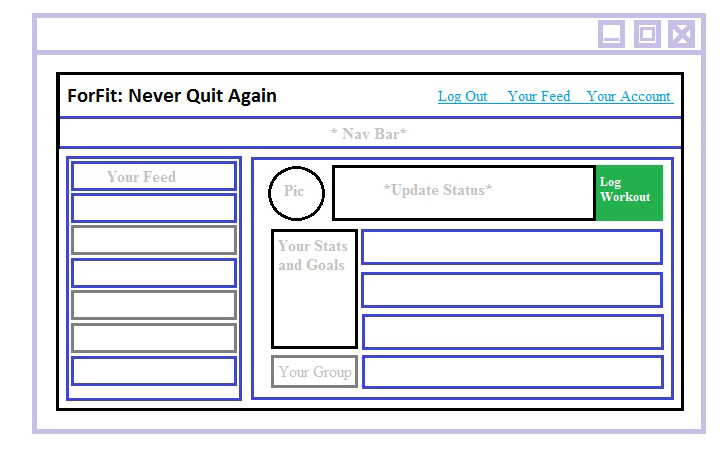
\includegraphics[width=\textwidth]{Wireframe.jpg}
\end{figure}

\end{document}